% class
\documentclass[a4paper,12pt,xelatex,ja=standard]{bxjsarticle}

% packages
%% mathematical notations
\usepackage{amsthm,amsmath,amssymb,amsfonts} % mathematical notations
\usepackage{bm} % bold character
\usepackage{latexsym} % more mathematical notations
\usepackage{physics} % physical notations
%% graphs
\usepackage{graphicx, xcolor} % graph
\usepackage{circuitikz} % for circuit elements
\usepackage{float} % positioning of graphs
\usepackage{siunitx} % SI units
\usepackage{tikz} % graphic elements
\usepackage{wrapfig} % must be after float package.
\usepackage{askmaps} % Karnaugh map
%% type system
\usepackage{bussproofs} % proof tree
%% code
\usepackage[ruled,vlined]{algorithm2e} % pseudo code
\usepackage{listings} % source code
\usepackage{inconsolata}
\lstset{
  basicstyle=\footnotesize,
  numbers=left,
  frame={tb}
}
\usetikzlibrary{automata, positioning}
\tikzset{
  ->,
  >={Stealth[round]},
  auto,
  every state/.style={draw}
}

% Basic information
\title{電子情報学専攻 \, 専門 \\ 平成20年 \, 解答・解説}
\author{diohabara}
\date{\today}

\begin{document}
\maketitle

\section*{第1問\ 電気・電子回路}

\section*{第2問\ 論理回路}
\subsection*{(1)}
下の図のような状態遷移図になる。

\begin{center}
  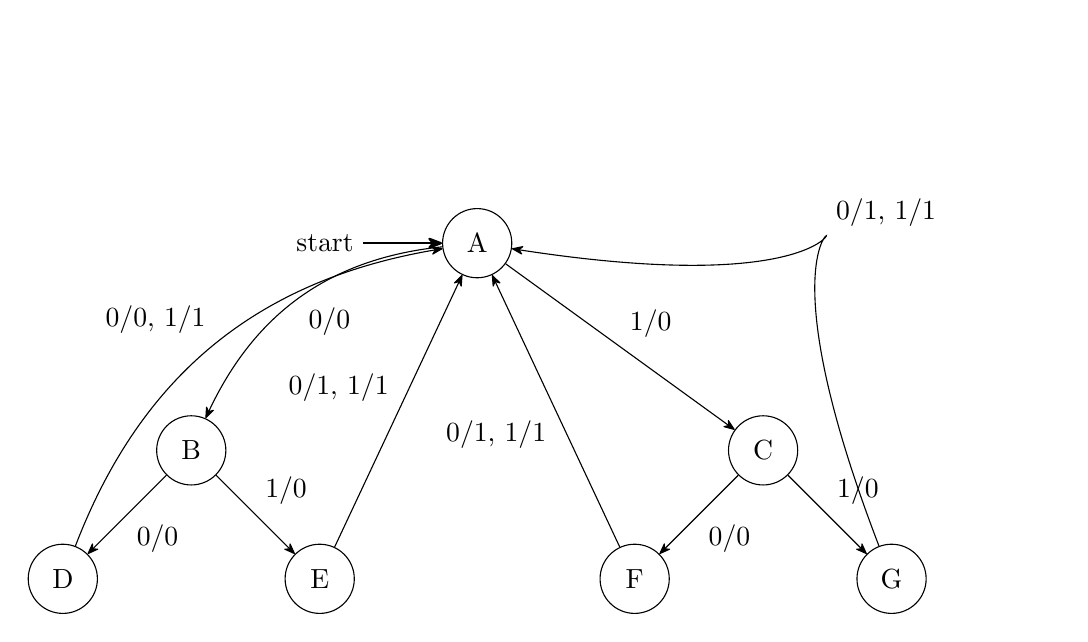
\begin{tikzpicture}
    \node[state] (A) {A};
    \node(left-A) [left=of A] {start};
    \draw[->, thick] (left-A) -- (A);
    \node[state] (B) [below left=2cm and 3cm of A] {B};
    \node[state] (C) [below right=2cm and 3cm of A] {C};
    \node[state] (D) [below left=of B] {D};
    \node[state] (E) [below right=of B] {E};
    \node[state] (F) [below left=of C] {F};
    \node[state] (G) [below right=of C] {G};

    \path
    (A)
      edge [bend right] node {0/0} (B)
      edge node {1/0} (C)
    (B)
      edge node {0/0} (D)
      edge node {1/0} (E)
    (C)
      edge node {0/0} (F)
      edge node {1/0} (G)
    (D)
      edge [bend left] node {0/0, 1/1} (A)
    (E)
      edge node {0/1, 1/1} (A)
    (F)
      edge node {0/1, 1/1} (A)
    (G)
      edge [bend right, looseness=3] node {0/1, 1/1} (A)
    ;
  \end{tikzpicture}
\end{center}

\subsection*{(2)}
同じ入力に対して同じ出力を返し、かつ同じ状態に遷移するようなノードをまとめると求める状態遷移図は以下の通り。

\begin{center}
  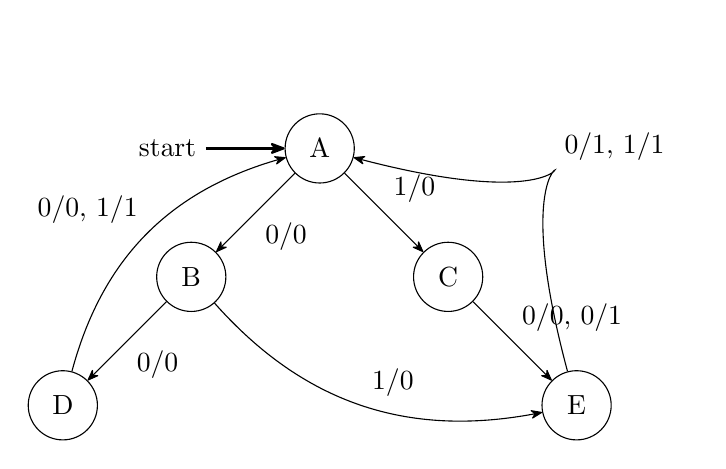
\begin{tikzpicture}
    \node[state] (A) {A};
    \node(left-A) [left=of A] {start};
    \draw[->, thick] (left-A) -- (A);
    \node[state] (B) [below left=of A] {B};
    \node[state] (C) [below right=of A] {C};
    \node[state] (D) [below left=of B] {D};
    \node[state] (E) [below right=of C] {E};

    \path
    (A)
      edge node {0/0} (B)
      edge node {1/0} (C)
    (B)
      edge node {0/0} (D)
      edge [bend right] node {1/0} (E)
    (C)
      edge node {0/0, 0/1} (E)
    (D)
      edge [bend left] node {0/0, 1/1} (A)
    (E)
      edge [bend right, looseness=3] node {0/1, 1/1} (A)
    ;
  \end{tikzpicture}
\end{center}

\subsection*{(3)}
状態遷移表は次の通り。ただし*は0でも1でも良いことを示す。
\begin{table}[H]
  \centering
  \begin{tabular}{|l|l|l|l|}
  \hline
  S & I & nextS & O \\ \hline \hline
  A & 0 & B     & 0 \\ \hline
  A & 1 & C     & 0 \\ \hline
  B & 0 & D     & 0 \\ \hline
  B & 1 & E     & 0 \\ \hline
  C & * & E     & 0 \\ \hline
  D & 0 & A     & 0 \\ \hline
  D & 1 & A     & 1 \\ \hline
  E & * & A     & 1 \\ \hline
  \end{tabular}
\end{table}

\subsection*{(4)}
入力を順にX,Y,Zとしてカルノー図は次の通り。
\begin{figure}[htbp]
  \centering
  \askmapiii{出力1}{{X}{Y}{Z}}{}{12345678}
  {
    \put(3.5, 1.0){\oval(1.8,1.8)[r]}%
    \put(3.5, 0.1){\line(-2, 0){3}}%
    \put(3.5, 1.9){\line(-2, 0){2}}%
    \put(0.5, 0.6){\oval(1.0, 1.0)[l]}%
    \put(1.4, 1.1){\oval(1.8, 1.7)[lt]}%
  }
  \caption{カルノー図}
\end{figure}

\subsection*{(5)}
TODO

\section*{第3問\ データベース}

\section*{第4問\ 信号処理}

\section*{第5問\ 情報通信}

\section*{第6問\ 統計学}

\end{document}

